\chapter{Experiments}
\label{ch:experiments}

\section{Datasets}
\label{sec:ds}

In this section we consider datasets that are separated in two opposing communities. The information about the opinions of each member of this community is known. Thus, we can assign internal opinions -1 and 1 to the nodes depending on their community membership\cite{tsapMatakosTerzi}.  We consider the following.

\begin{enumerate}

  \item The Karate dataset, that represents the friendships between the members of a karate club at a US university. This network is split in two equal size polarized communities around two rival karate instructors.
  
  \item The Books dataset, that is a network of US politics books. These books were published near the 2004 presidential election and sold by Amazon.com . These Books are classified as "Liberal", "Conservative", or "Neutral".
  
  \item The Blogs dataset. A network of hyperlinks between online blogs on US politics.
  
\end{enumerate}
\section{Experiments with heuristics}
\label{sec:experimHeuristics}

 We evaluate the heuristic algorithms by comparing them with the Greedy  algorithm. 

\begin{figure}[!htbp]
	\centering
	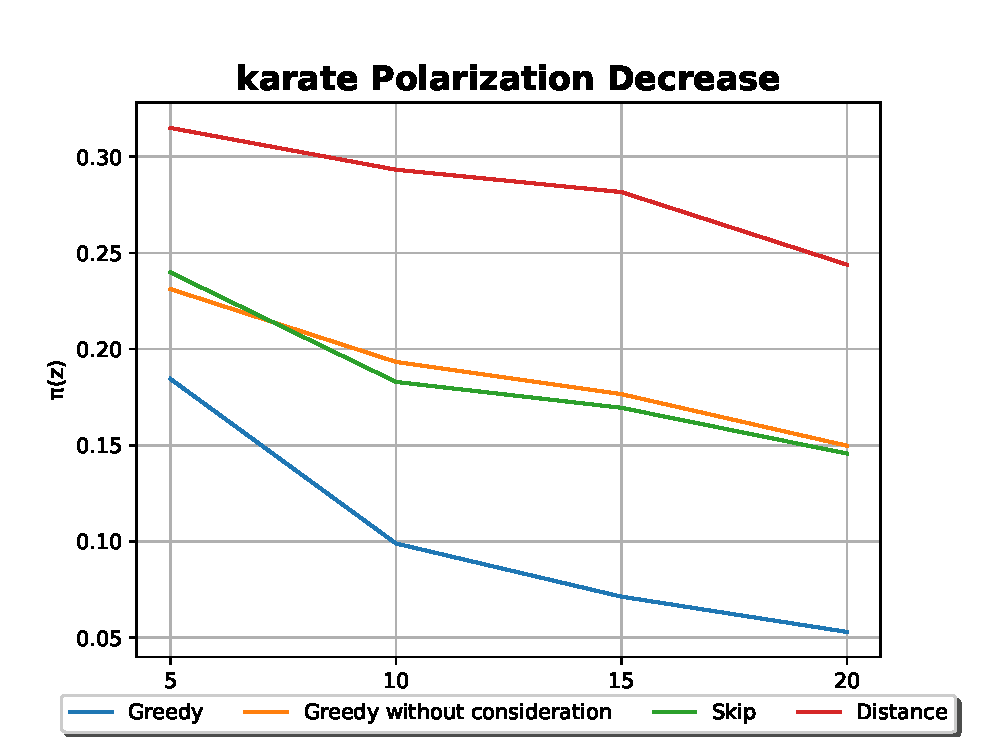
\includegraphics[width=0.65\textwidth]{Figures/karate_pol}
	\caption{Heuristic comparison of the decrease in Karate}
	\label{fig:karate_pol}
\end{figure}


\begin{figure}[!htbp]
	\centering
	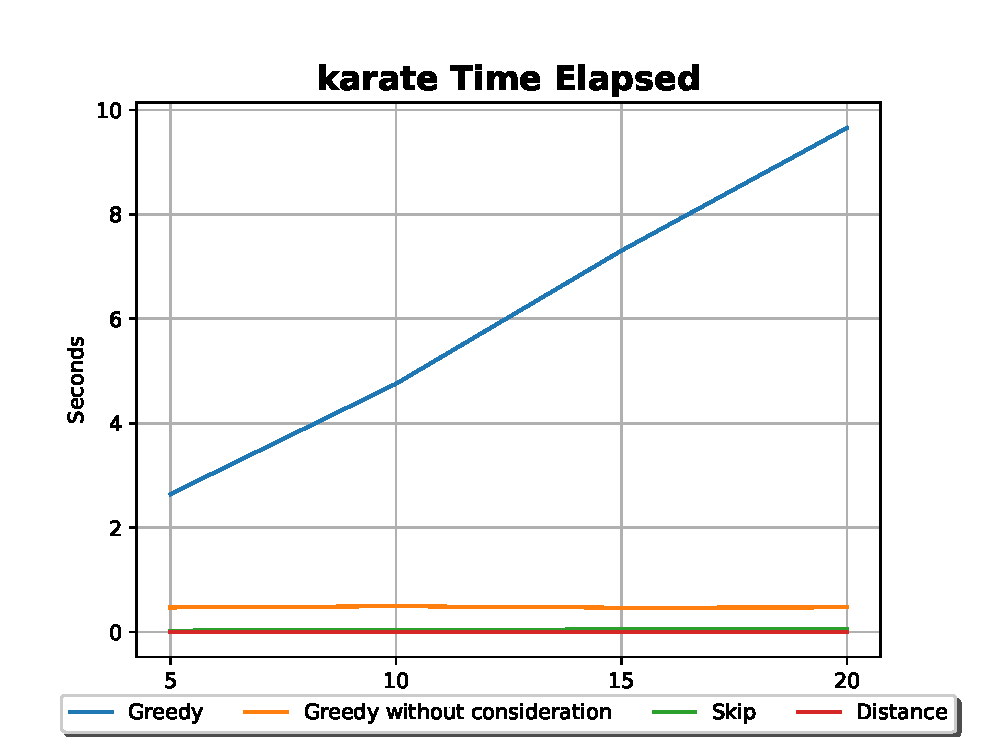
\includegraphics[width=0.65\textwidth]{Figures/karate_time}
	\caption{Heuristic comparison of time in Karate}
	\label{fig:karate_time}
\end{figure}



\begin{figure}[!htbp]
	\centering
	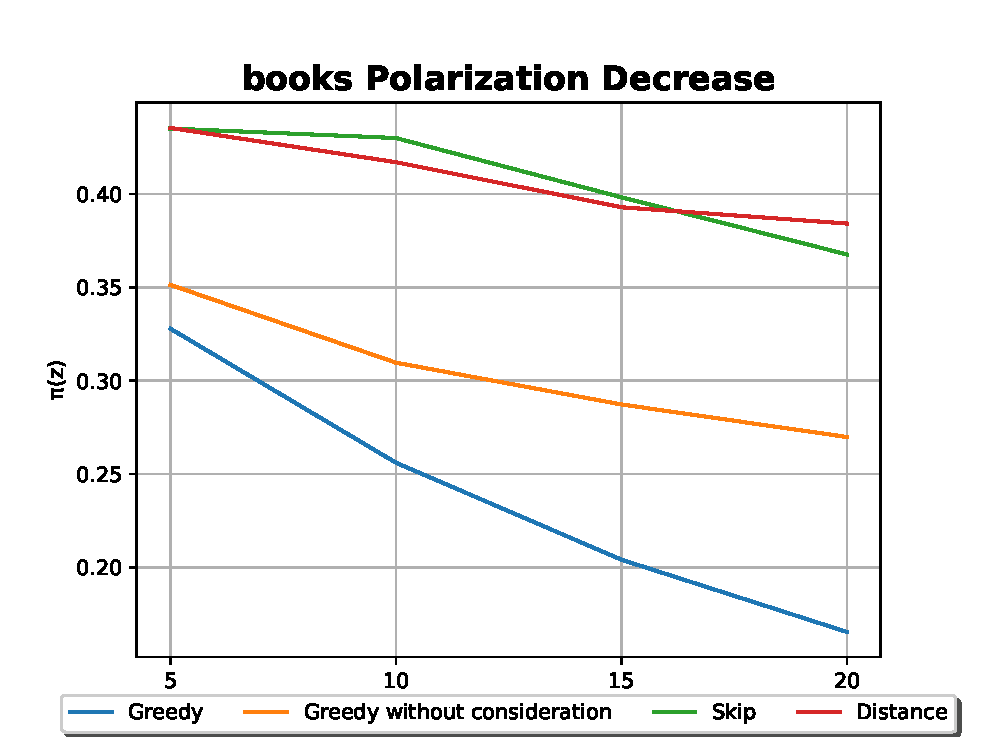
\includegraphics[width=0.65\textwidth]{Figures/books_pol}
	\caption{Heuristic comparison of the decrease}
	\label{fig:books_pol}
\end{figure}


\begin{figure}[!htbp]
	\centering
	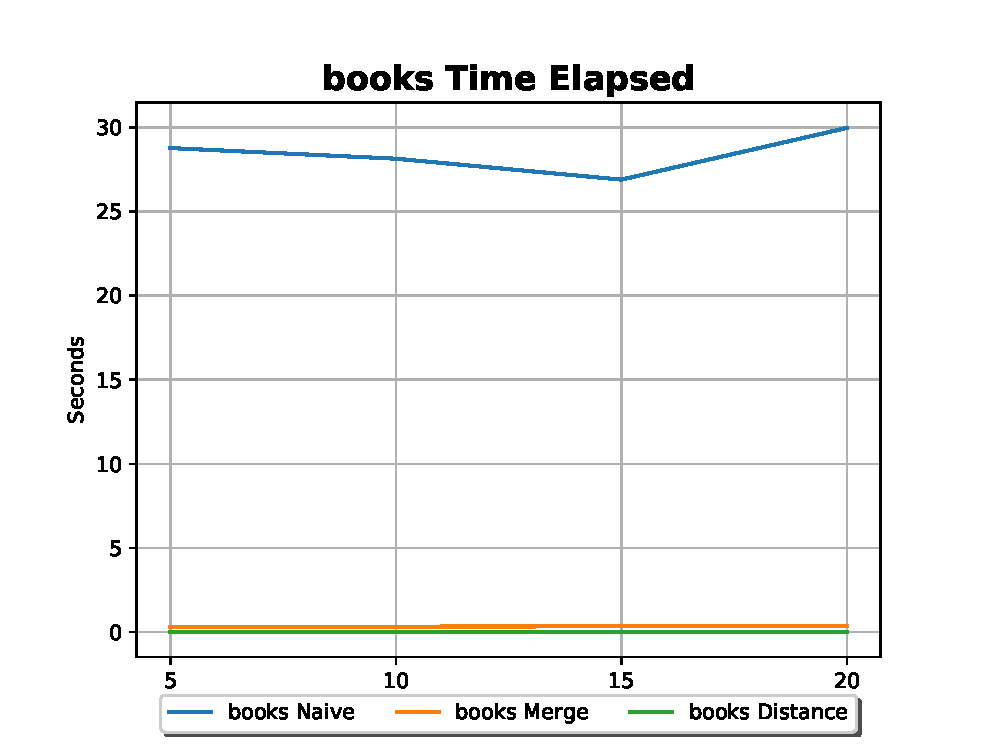
\includegraphics[width=0.65\textwidth]{Figures/books_time}
	\caption{Heuristic comparison of time}
	\label{fig:books_time}
\end{figure}



\section{Polarization in a complete graph}
\label{sec:fullgraph}
\vspace{20pt}
Given a polarized graph $G$ we will compute the polarization index $\pi(z)$ before and after converting the graph $G$ to a full graph. 

\begin{table}[!htbp]
 \centering
 \caption{Polarization Before and after converting to a full graph}
 \label{tab:fullgraph}
 \begin{tabular}{| l || l | l | l | l |}
 \hline
  Dataset & Number of Nodes & Number of edges & Average Degree & $\pi(z)$\\
  \hline
  \hline
  Karate Before & $34$ & $78$ & $4.5882$ &  $0.35857$\\
  \hline
  Karate After & $34$ & $561$ & $33$ &  $0.00081$\\
  \hline
  \hline
  Books Before & $105$ & $441$ & $8.4000$ &  $0.44046$\\
  \hline
  Books After & $105$ & $5460$ & $104.0000$ &  $0.00453$\\
  \hline
  \hline
  Blogs Before & $1490$ & $16718$ & $22.4403$ &  $0.27909$\\
  \hline
  Blogs After & $1490$ & $1109308$ & $1489.0040$ &  $0.00030$\\
  \hline
 \end{tabular}
 \end{table}

\vspace{20pt}
\noindent
We can see the results from the karate, books and blogs datasets at table ~\ref{tab:fullgraph}. The results leads us to the following lemma.
\\	
\begin{lemma}
The polarization index does not necessarily drops to zero in a fully connected graph.
\end{lemma}


\section{Polarization decrease by removing edges}
\label{sec:polremovingdecrease}
Bellow we examine the removal of edges from a social graph and their result in polarization. We also find the edge betweenness centrality of each edge. 
\\
\\
The edge betweenness centrality is defined as the number of the shortest paths that go through an edge in a graph or network.(add cite Girvan and Newman 2002). 
\\
\\
In the tables following, Sign and Addition refer to the multiplication and the addition of the opinions of the nodes that are attached to the specific edge examined. Graphs in the books and blogs datasets, due to size, are omitted.
\\
\\

\subsection{Edges removal in the Karate dataset}

\begin{table}[H]
 \centering
 \caption{Edges with the biggest increase of polarization}
 \label{tab:edgesLargest}
 \begin{tabular}{| l || l | l | l | l |}
 \hline
  Edge & Betweenness Centrality & Polarization Increase & Sign & Addition\\
  \hline
  \hline
  (1, 32) & $0.12725$ & $0.04669$ & - &  0\\
  \hline
  (20, 34) & $0.059384$ & $0.03470$ & - &  0\\
  \hline
  (14, 34) & $0.06782$ & $0.02924$ & - &  0\\
  \hline
  (2, 31) & $0.03228$ & $0.02505$ & - &  0\\
  \hline
  (3, 28) & $0.04119$ & $0.02068$ & - &  0\\
  \hline
 \end{tabular}
  
 \caption{Edges with the biggest decrease of polarization }
 \label{tab:edgesLargest}
 \begin{tabular}{| l || l | l | l | l |}
 \hline
  Edge & Betweenness Centrality & Polarization Decrease & Sign & Addition\\
  \hline
  \hline
  (5, 11) & $0.00297$ & $5.55111*10^{-17}$ & + &  -2\\
  \hline
  (4, 8) & $0.00336$ & $3.04869*10^{-7}$ & + &  -2\\
  \hline
  (1, 4) & $0.02049$ & $1.38023*10^{-5}$ & + &  -2\\
  \hline
  (32, 34) & $0.05339$ & $1.61826*10^{-5}$ & + &  +2\\
  \hline
  (1, 8) & $0.02282$ & $1.93446*10^{-5}$ & + &  -2\\
  \hline
  \hline
 \end{tabular}
\end{table}

\begin{figure}[H]
	\centering
	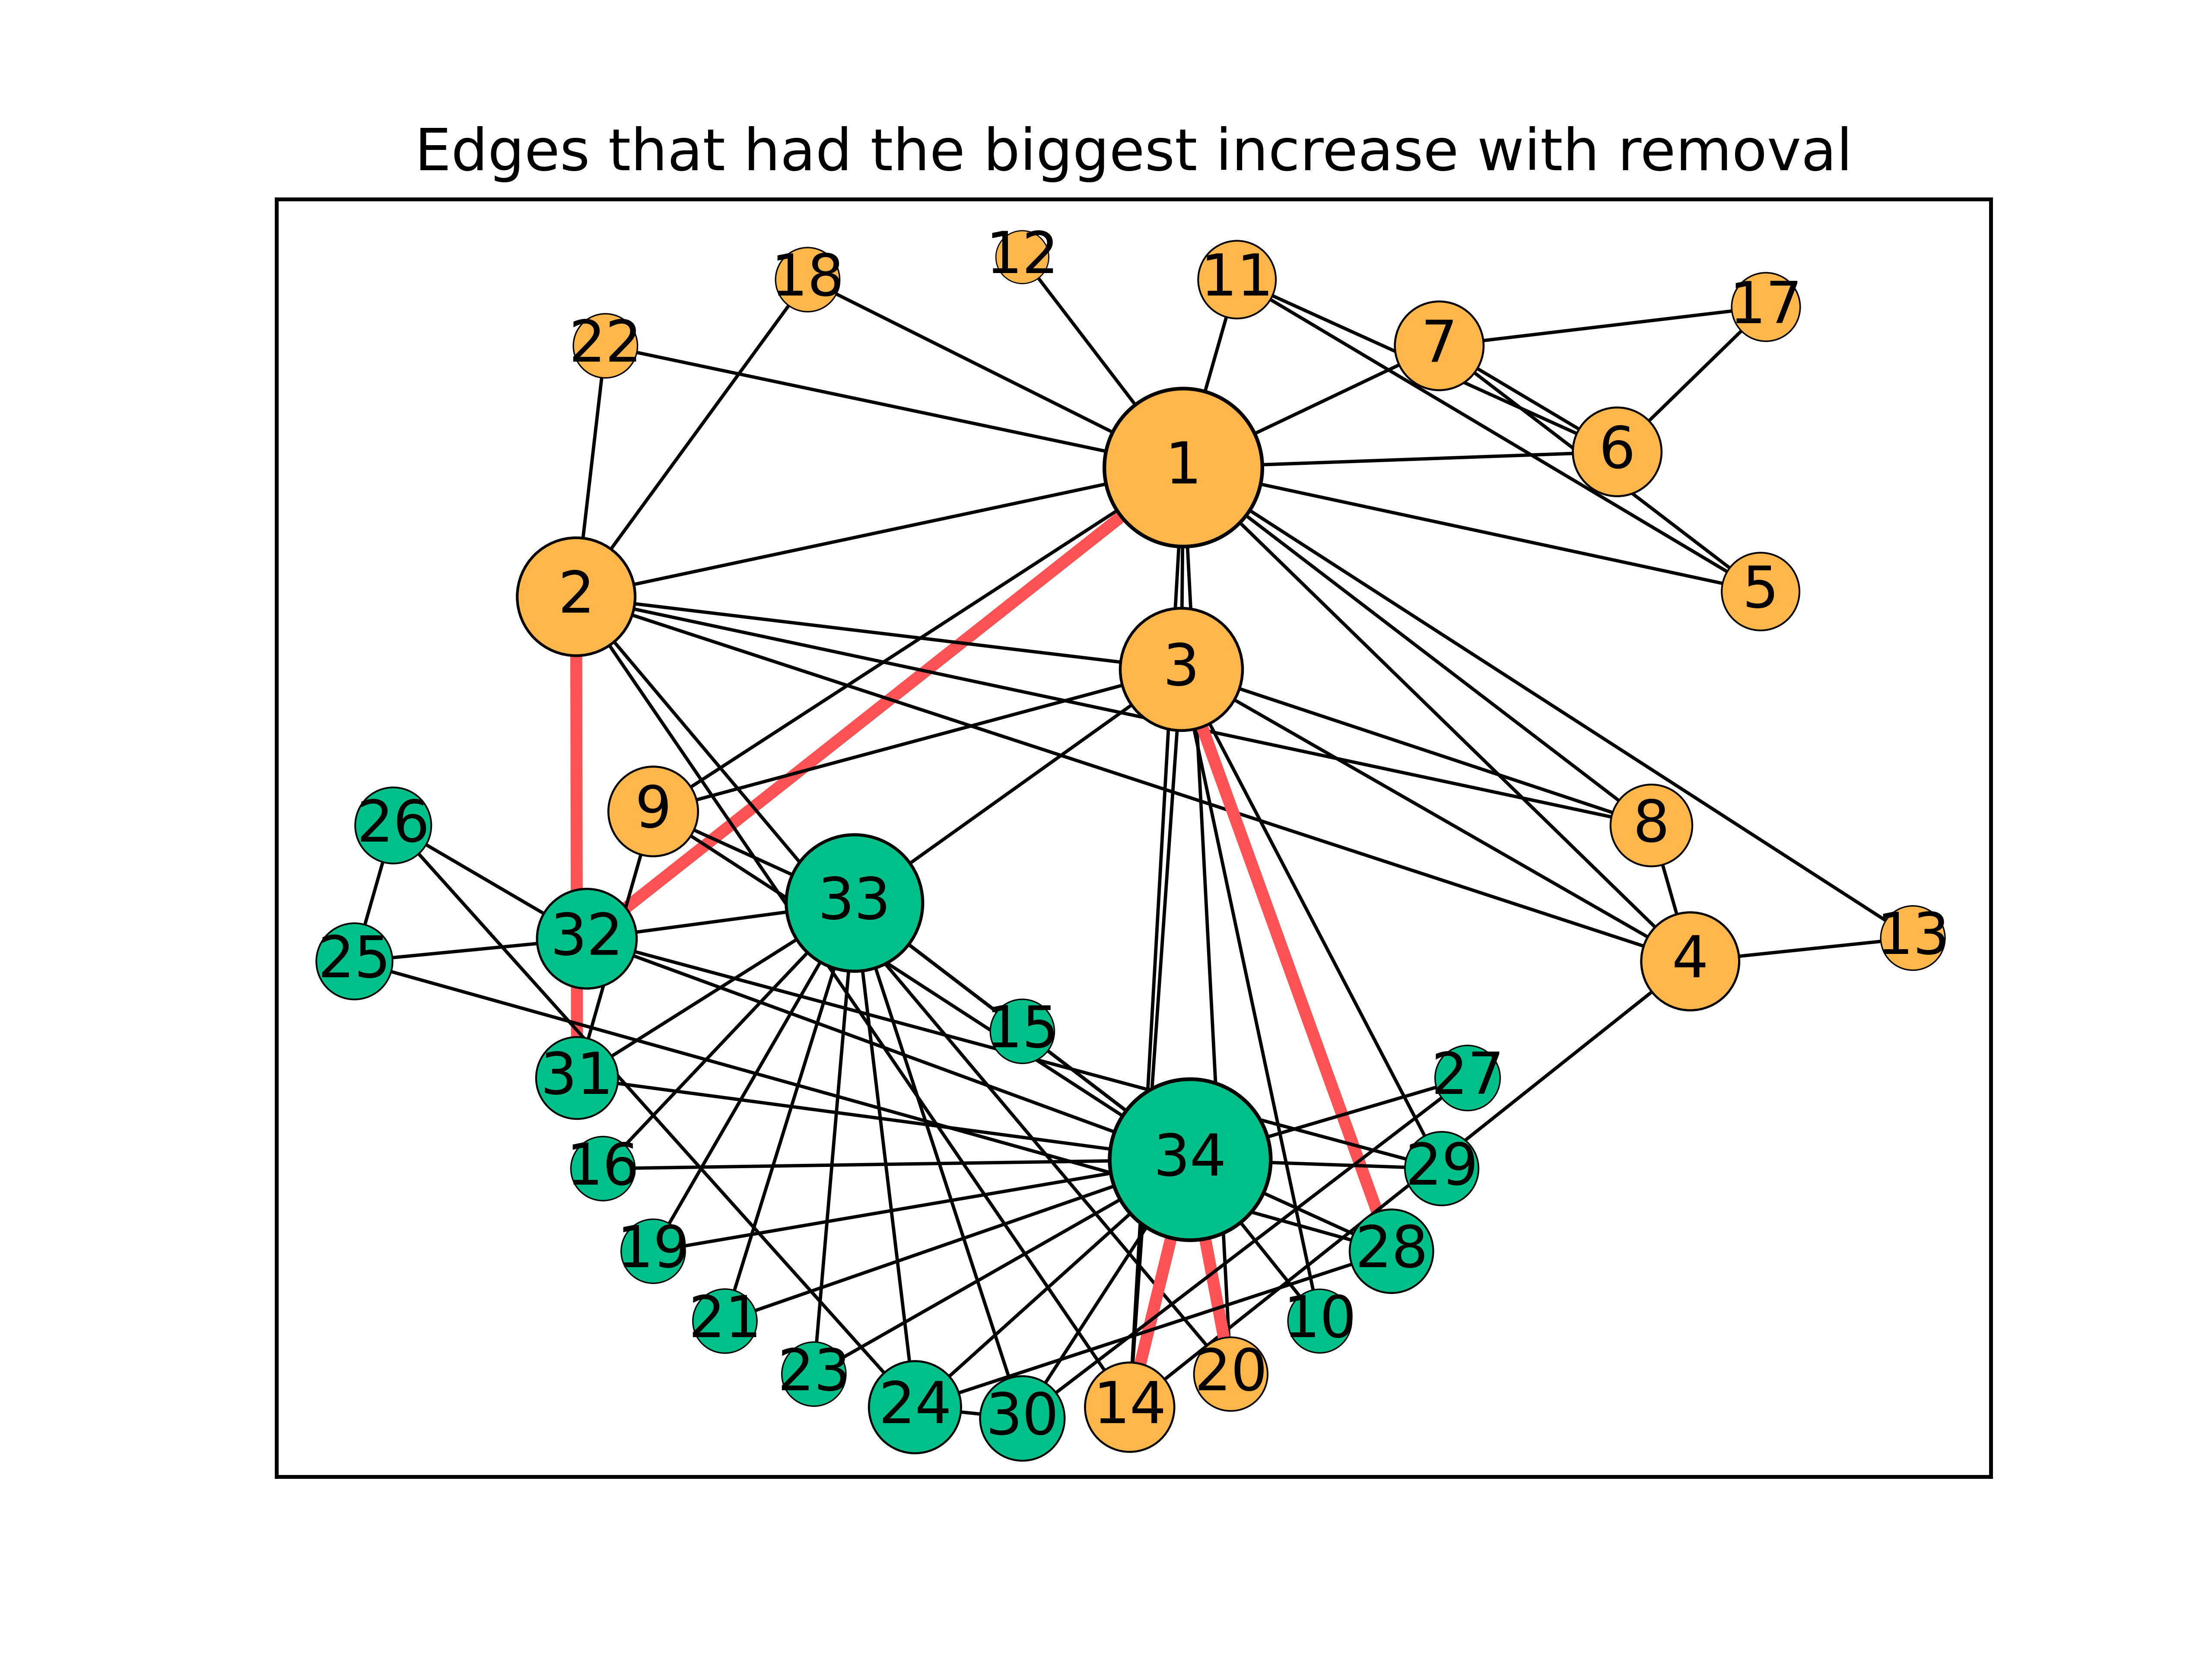
\includegraphics[width=0.65\textwidth]{Figures/karate_increase}
	\label{fig:karate_increase}
	\caption{Removing edges in Karate}
\end{figure}

\begin{figure}[H]
	\centering
	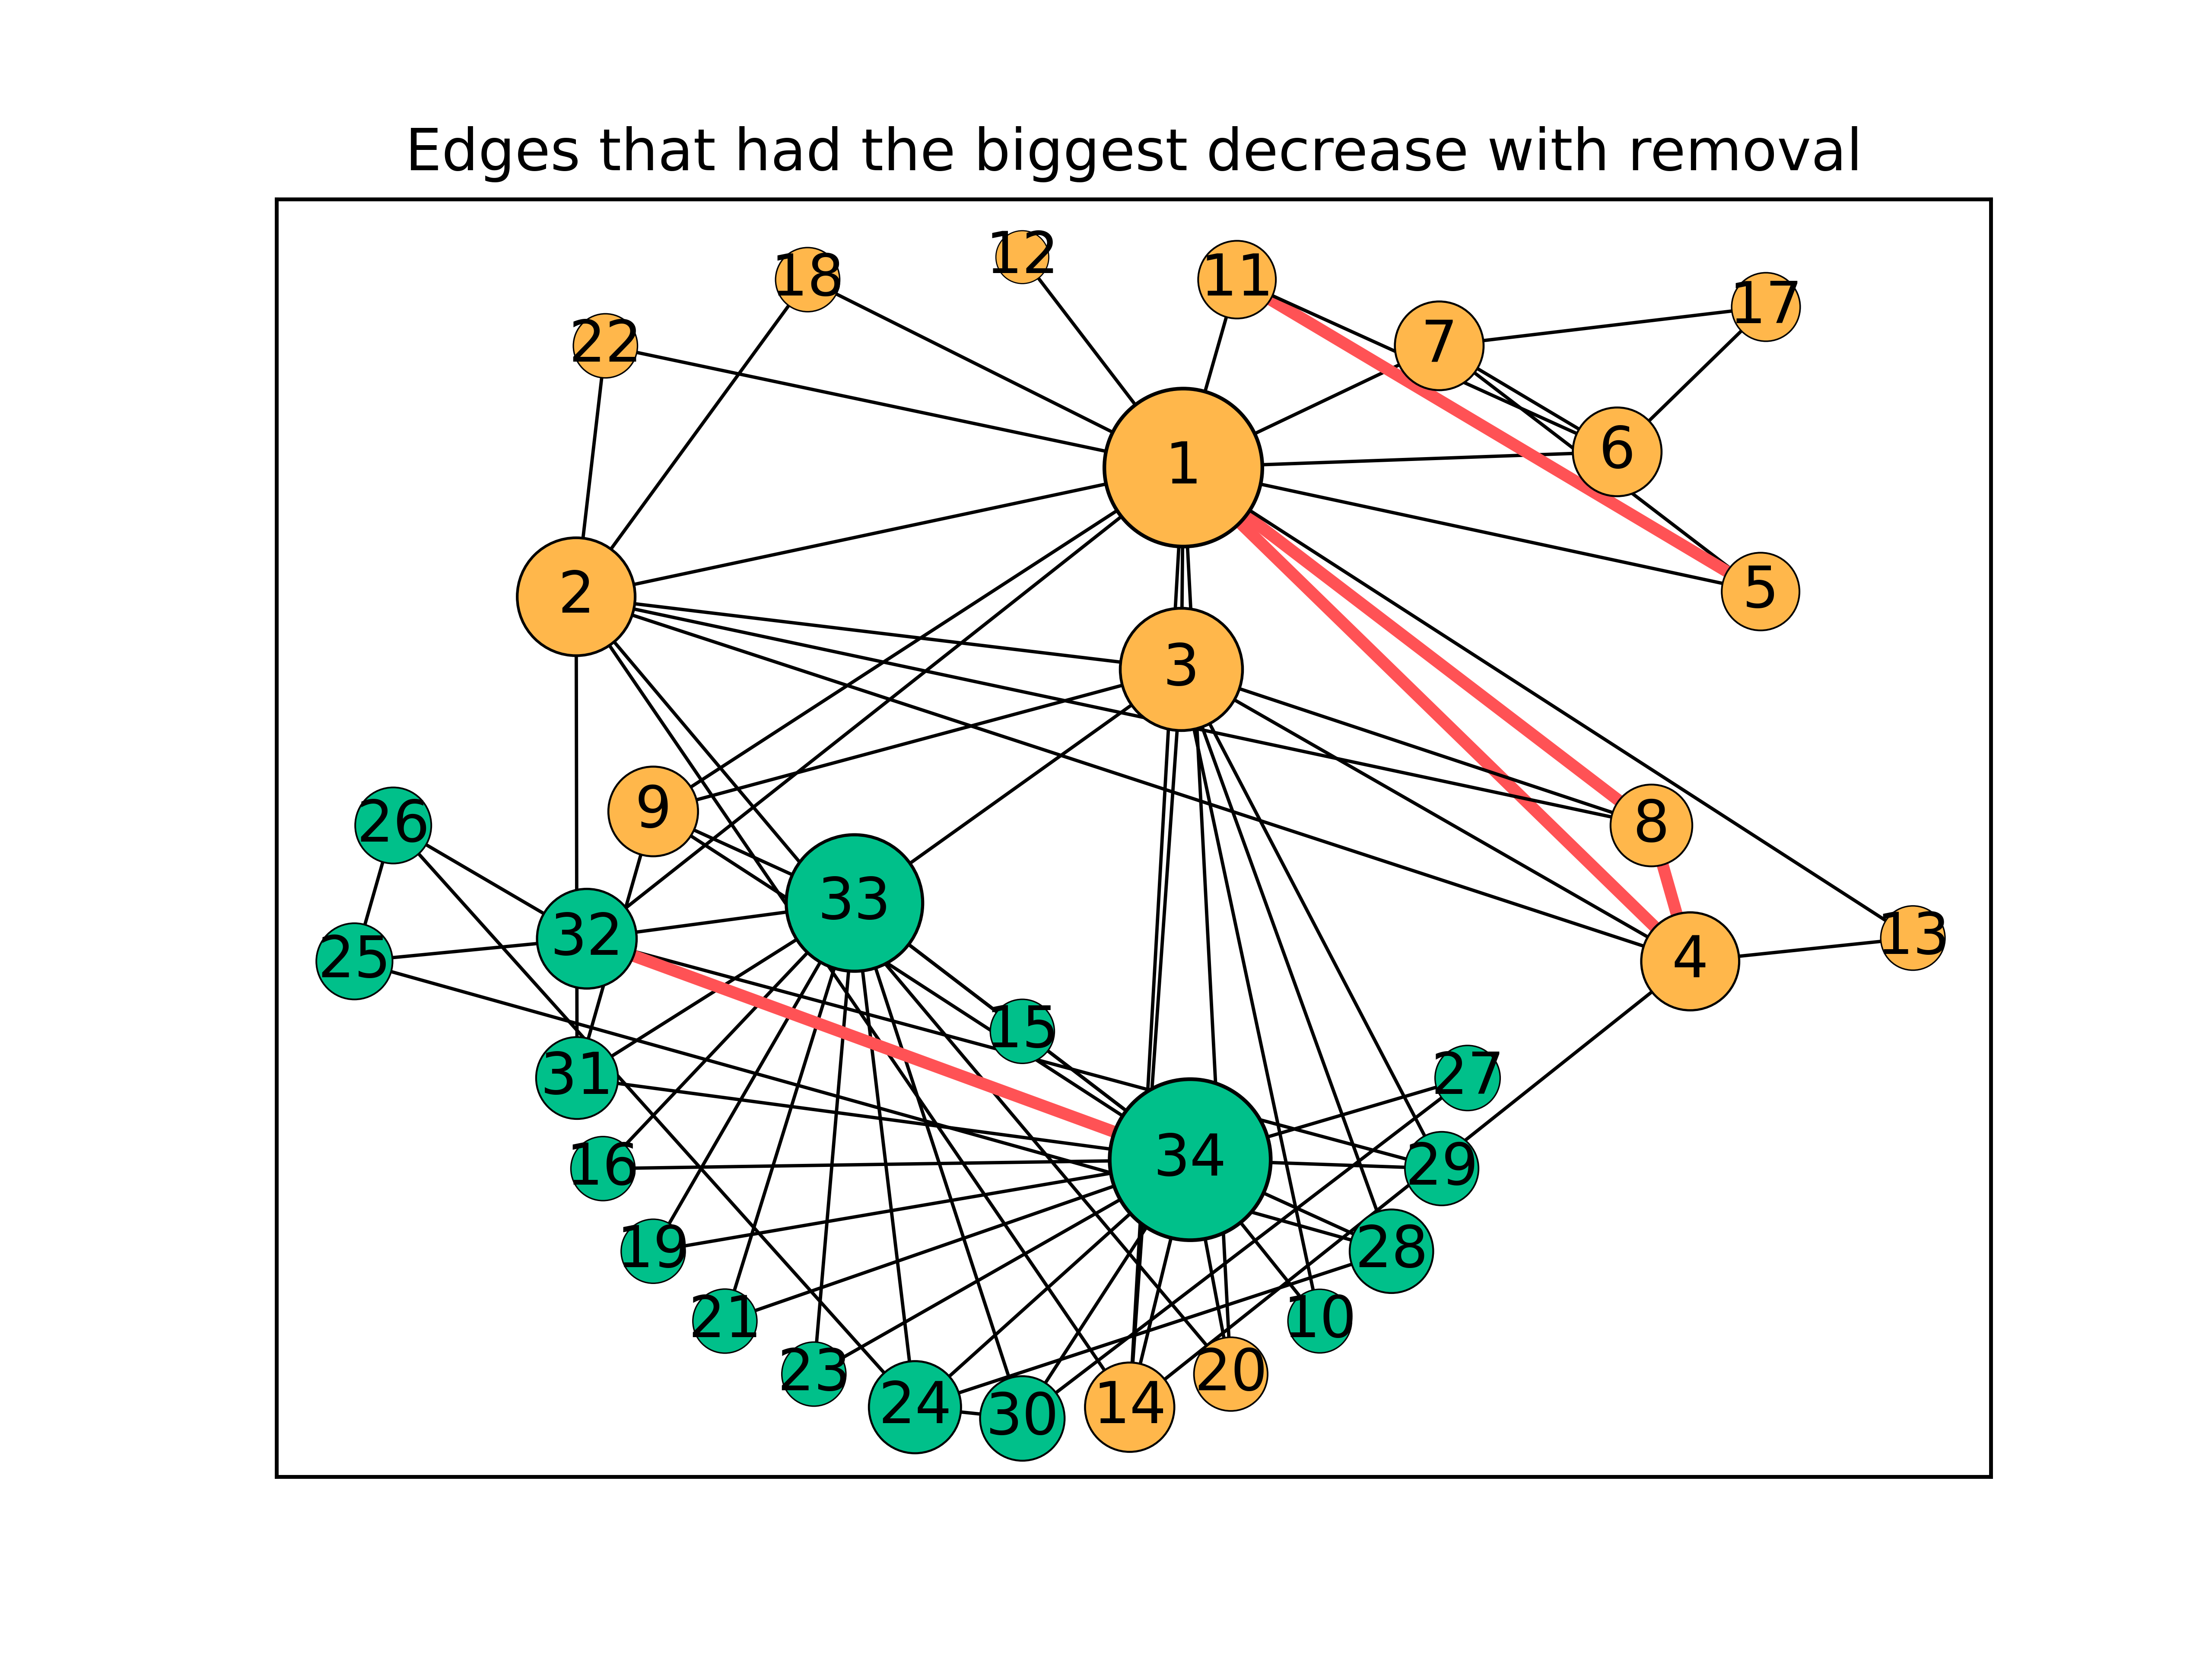
\includegraphics[width=0.65\textwidth]{Figures/karate_decrease}
	\label{fig:karate_decrease}
	\caption{Removing edges in Karate}
\end{figure}


\subsection{Edges removal in the Blogs dataset}

\begin{table}[H]
 \centering
 \caption{Edges with the biggest increase of polarization}
 \label{tab:edgesLargest}
 \begin{tabular}{| l || l | l | l | l |}
 \hline
  Edge & Betweenness Centrality & Polarization Increase & Sign & Addition\\
  \hline
  \hline
  (213, 793) & $0.00219$ & $0.00091$ & - &  0\\
  \hline
  (600, 1183) & $0.00439$ & $0.00074$ & - &  0\\
  \hline
  (523, 1375) & $0.00110$ & $0.00070$ & - &  0\\
  \hline
  (325, 1159) & $0.00110$ & $0.00069$ & - &  0\\
  \hline
  (632, 1000) & $0.00110$ & $0.00069$ & - &  0\\
  \hline
 \end{tabular}
 
 
 \caption{Edges with the biggest decrease of polarization }
 \label{tab:edgesLargest}
 \begin{tabular}{| l || l | l | l | l |}
 \hline
  Edge & Betweenness Centrality & Polarization Decrease & Sign & Addition\\
  \hline
  \hline
  (574, 1380) & $0.00014$ & $2.09620*10^{-6}$ & - &  0\\
  \hline
  (23, 1380) & $0.00021$ & $2.18102*10^{-6}$ & - &  0\\
  \hline
  (600, 1021) & $0.00024$ & $2.41460*10^{-6}$ & - &  0\\
  \hline
  (634, 1380) & $0.00010$ & $2.60119*10^{-6}$ & - &  0\\
  \hline
  (219, 1380) & $0.00014$ & $2.91467*10^{-6}$ & - &  0\\
  \hline
  \hline
 \end{tabular}
 
\end{table}

\subsection{Edges removal in the Books dataset}
\begin{table}[H]
 \centering
 \caption{Edges with the biggest increase of polarization }
 \label{tab:edgesLargest}
 \begin{tabular}{| l || l | l | l | l |}
 \hline
  Edge & Betweenness Centrality & Polarization Increase & Sign & Addition\\
  \hline
  \hline
  (0, 5) & $0.00056$ & $2.65885*10^5$ & - &  0\\
  \hline
  (7, 58) & $0.00713$ & $0.00012$ & - &  0\\
  \hline
  (5, 6) & $0.00222$ & $0.00012$ & - &  0\\
  \hline
  (6, 18) & $0.00858$ & $0.00014$ & +& -2\\
  \hline
  (0, 2) & $0.00031$ & $0.00349$ & - &  0\\
  \hline
 \end{tabular}
\end{table}

\begin{table}[H]
 \centering
 \caption{Edges with the biggest decrease of polarization}
 \label{tab:edgesLargest}
 \begin{tabular}{| l || l | l | l | l |}
 \hline
  Edge & Betweenness Centrality & Polarization Decrease & Sign & Addition\\
  \hline
  \hline
  (53, 76) & $0.06290$ & $0.01985$ & - &  0\\
  \hline
  (46, 102) & $0.04914$ & $0.01541$ & + &  -2\\
  \hline
  (19, 77) & $0.04367$ & $0.01458$ & + &  +2\\
  \hline
  (9, 51) & $0.02812$ & $0.01000$ & - &  0\\
  \hline
  (49, 72) & $0.06809$ & $0.00952$ & - &  0\\
  \hline
 \end{tabular} 
\end{table}

\subsection{Remarks about the edge removals}

We can clearly see that there is an association between the edge betweenness centrality and the decrease in polarization. Edges that contribute to a bigger decrease have larger betweenness centrality. 
\\
\\
A second thing that we see in all three datasets is that the biggest increase is coming from the removal of edges that connect opposing opinions.
\\
\\
In addition, during the experiments on the karate dataset, the removal of edge $(6, 7)$ had no effect on the polarization index. This leads to the following lemma.

\begin{lemma}
The polarization index can stay the same after an edge removal.
\end{lemma}

